\subsection{Pengukuran Kuantum}
Pengukuran merupakan tahap yang menghubungkan informasi kuantum dengan hasil observasi klasik yang dapat diakses oleh pengguna. Dalam mekanika kuantum, setiap besaran fisik direpresentasikan oleh suatu operator observabel Hermitian $\hat{O}$ yang memiliki himpunan nilai eigen $o_n$ dan vektor eigen ortonormal $|e_n\rangle$. Hubungan antara observabel dan basis eigennya dinyatakan melalui persamaan
\begin{equation}
\hat{O}|e_n\rangle = o_n |e_n\rangle.
\end{equation}
Jika suatu sistem berada pada keadaan $|\psi\rangle$, maka hasil pengukuran yang mungkin diperoleh hanyalah nilai-nilai eigen dari operator observabel tersebut. Untuk sebuah qubit yang berada pada keadaan superposisi
\begin{equation}
|\psi\rangle = a|0\rangle + b|1\rangle,
\end{equation}
probabilitas diperolehnya suatu hasil pengukuran ditentukan oleh kaidah Born (\textit{Born rule}). tersebut menyatakan bahwa probabilitas untuk memperoleh nilai eigen $o_n$ diberikan oleh proyeksi keadaan terhadap basis eigen observabel,
\begin{equation}
P(o_n) = |\langle e_n|\psi\rangle|^2.
\end{equation}
Sehingga, pada basis komputasi, probabilitas diperolehnya keadaan $|0\rangle$ dan $|1\rangle$ menjadi
\begin{equation} P(0)=|a|^2, \qquad P(1)=|b|^2.
\end{equation}
Hal tersebut menginterpretasi probabilistik ini menunjukkan bahwa hasil pengukuran tidak dapat diprediksi secara deterministik untuk satu percobaan tunggal, melainkan hanya dapat diprediksi melalui distribusi probabilitas hasil pengukuran.

Secara matematis, proses pengukuran direpresentasikan menggunakan operator proyeksi
\begin{equation} \hat{P}_n = |e_n\rangle\langle e_n|.
\end{equation}
Jika hasil pengukuran yang diperoleh adalah nilai eigen $o_n$, maka keadaan sistem setelah pengukuran diberikan oleh
\begin{equation}
|\psi'\rangle = \frac{\hat{P}_n|\psi\rangle} {\sqrt{\langle\psi|\hat{P}_n|\psi\rangle}}.
\end{equation}
Persamaan tersebut menunjukkan bahwa pengukuran menyebabkan sistem kehilangan superposisinya dan bertransisi menuju salah satu keadaan eigen observabel. Fenomena tersebut dikenal sebagai keruntuhan keadaan kuantum (\textit{state collapse}), yaitu perubahan non-unitari dari superposisi beberapa kemungkinan hasil menuju satu keadaan yang terdefinisi secara pasti~\shortcite{tomaz_quantum_2025}. Mekanisme fisik yang menyebabkan hilangnya interferensi kuantum dapat dipahami melalui representasi matriks densitas~\cite{revythi_quantum_2025}. Untuk keadaan murni
\begin{equation}
|\psi\rangle = a|0\rangle+b|1\rangle,
\end{equation}
matriks densitas sistem didefinisikan sebagai
\begin{equation}
\rho = |\psi\rangle\langle\psi|.
\end{equation}
Dengan melakukan perkalian luar (\textit{outer product}), diperoleh
\begin{equation}
\begin{split}
\rho &= (a|0\rangle+b|1\rangle) (a^*\langle0|+b^*\langle1|)\\
&= |a|^2|0\rangle\langle0|+ ab^*|0\rangle\langle1| + a^*b|1\rangle\langle0| + |b|^2|1\rangle\langle1|.
\end{split}
\end{equation}
Dalam basis komputasi, bentuk tersebut dapat dituliskan sebagai
\begin{equation}
\rho=
\begin{bmatrix}
|a|^2 & ab^*\\
a^*b & |b|^2
\end{bmatrix}
\end{equation}
di mana elemen diagonal menyatakan probabilitas populasi masing-masing keadaan basis, sedangkan elemen \textit{off-diagonal} merepresentasikan koherensi kuantum yang bertanggung jawab terhadap fenomena interferensi.

Pada dasarnya, sistem kuantum tidak pernah sepenuhnya terisolasi dari lingkungan~\shortcite{li_quantum_2025}. Ketika sistem berinteraksi dengan lingkungan, keadaan gabungan sistem-lingkungan dapat dituliskan sebagai
\begin{equation}
|\Psi\rangle
=
a|0\rangle|e_0\rangle
+
b|1\rangle|e_1\rangle.
\end{equation}
Matriks densitas sistem kemudian diperoleh melalui operasi \textit{partial trace} terhadap derajat kebebasan lingkungan,
\begin{equation}
\rho_S
=
\mathrm{Tr}_E
\left(
|\Psi\rangle\langle\Psi|
\right),
\end{equation}
yang menghasilkan
\begin{equation}
\rho_S=
\begin{bmatrix}
|a|^2 &
ab^*\langle e_1|e_0\rangle\\
a^*b\langle e_0|e_1\rangle &
|b|^2
\end{bmatrix}.
\end{equation}
Keberadaan faktor $\langle e_1|e_0\rangle$ menunjukkan bahwa koherensi sistem bergantung pada tingkat tumpang tindih keadaan lingkungan yang berkorelasi dengan masing-masing keadaan basis qubit. Namun seiring bertambahnya interaksi dengan lingkungan, keadaan lingkungan menjadi semakin ortogonal sehingga
\begin{equation}
\langle e_1|e_0\rangle
\rightarrow 0.
\end{equation}
Sehingga elemen-elemen \textit{off-diagonal} menghilang dan matriks densitas sistem mereduksi menjadi
\begin{equation}
\rho_S
\rightarrow
\begin{bmatrix}
|a|^2 & 0\\
0 & |b|^2
\end{bmatrix}.
\end{equation}
Proses hilangnya koherensi kuantum ini dikenal sebagai dekoherensi (\textit{decoherence}) yaitu mengubah keadaan kuantum menjadi campuran statistik yang tidak lagi menunjukkan interferensi.

Secara konsep, hubungan antara dekoherensi dan keruntuhan keadaan kuantum tersebut dapat direpresentasikan pada Gambar \ref{fig:collapse_measurement}. Gambar tersebut memperlihatkan bagaimana elemen \textit{off-diagonaal} yang merepresentasikan koherensi kuantum secara bertahap menghilang akibat interaksi dengan lingkungan, menghasilkan matriks densitas diagonal yang bersifat statistik~\shortcite{anshu_sample-efficient_2020}. Setelah itu, proses pengukuran memproyeksikan sistem ke salah satu keadaan basis yang terdefinisi secara pasti sesuai probabilitas yang diberikan oleh kaidah Born~\shortcite{benedetti_parameterized_2019}.

\begin{figure}[htbp]
    \centering
    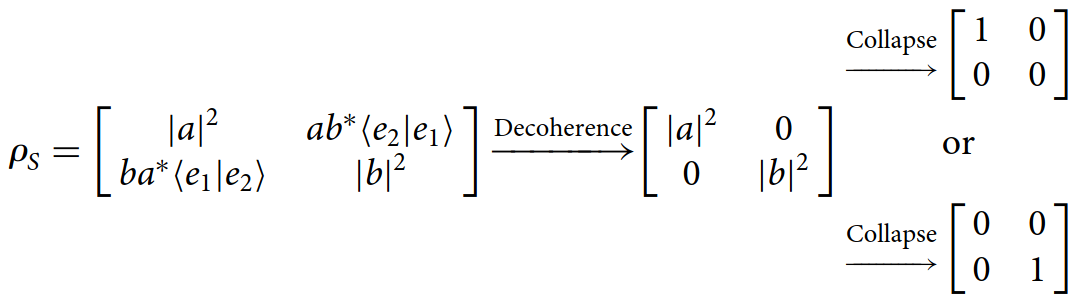
\includegraphics[width=\textwidth]{Images/Collapse_Measurement.png}
    \caption{Representasi konseptual hubungan antara dekoherensi dan keruntuhan keadaan kuantum. Interaksi sistem dengan lingkungan menyebabkan hilangnya elemen koherensi (\textit{off-diagonaal}) pada matriks densitas, sedangkan proses pengukuran memproyeksikan sistem ke salah satu keadaan eigen yang terdefinisi.}
    \label{fig:collapse_measurement}
\end{figure}